\documentclass{beamer}

\mode<presentation> {
\usetheme[secheader]{Madrid}
\usecolortheme{seahorse}
\useinnertheme{circles}
}

\usepackage{graphicx} % Allows including images
\usepackage{booktabs} % Allows the use of \toprule, \midrule and \bottomrule in tables
\usepackage{tikz}
\usepackage{caption}
\usepackage{hyperref}



%----------------------------------------------------------------------------------------
%	TITLE PAGE
%----------------------------------------------------------------------------------------

\title[Course Administration]{Course Administration} % The short title appears at the bottom of every slide, the full title is only on the title page

\author{Chaklam Silpasuwanchai} % Your name
\institute[AIT] % Your institution as it will appear on the bottom of every slide, may be shorthand to save space
{
Asian Institute of Technology \\ % Your institution for the title page
\medskip
\textit{chaklam@ait.asia} % Your email address
}
\date{} % Date, can be changed to a custom date

\begin{document}

\begin{frame}
\titlepage % Print the title page as the first slide
\end{frame}

\begin{frame}
\frametitle{Overview} % Table of contents slide, comment this block out to remove it
\tableofcontents % Throughout your presentation, if you choose to use \section{} and \subsection{} commands, these will automatically be printed on this slide as an overview of your presentation
\end{frame}

%----------------------------------------------------------------------------------------
%	PRESENTATION SLIDES
%----------------------------------------------------------------------------------------

%------------------------------------------------
%------------------------------------------------

\section{Administration} % A subsection can be created just before a set of slides with a common theme to further break down your presentation into chunks

\begin{frame}
\frametitle{Administration}
\begin{itemize}
	\item Course materials at \underline{\href{https://drive.google.com/drive/folders/1cHWrCKnRc1_xkWr_IgW4X-iBqm1hsnhP?usp=sharing}{Google Drive}} or \underline{\url{chaklam.com}}
	\item Google Classroom (Code: in the class)
	\item Email: \underline{\href{mailto:chaklam@ait.asia}{chaklam@ait.asia}} 
	\item Office hours: see my calendar chaklam@ait.asia
\end{itemize}
\vspace{0.2cm}
Let's have a short tour to chaklam.com,  Google Drive,  and Google classroom.
\end{frame}

\section{Why and what} % A subsection can be created just before a set of slides with a common theme to further break down your presentation into chunks

\begin{frame}
\frametitle{Why and what HCI}
\begin{itemize}
	\item HCI is \textbf{pervasive} and \textbf{multi-disciplinary}
	\begin{itemize}
		\item User Interface
		\item Input Devices: Mouse, Keyboard, Stylus, etc.
		\item Applications
	\end{itemize}
	\item Key goals
	\begin{itemize}
		\item Reliability $\rightarrow$ Productivity $\rightarrow$ Creativity \\  $\rightarrow$ Engagement $\rightarrow$ \textbf{Well-Being }
	\end{itemize}
	\item Research Areas
	\begin{itemize}
		\item User Experience and Usability
		\item Education, Health, Aging, Game applications
		\item Interaction - VR, AR, Haptics, Pen, Eye, Voice, Gesture, Textiles, Brain, etc.
		\item Understanding People
	\end{itemize}
	\item Research Questions
	\begin{itemize}
		\item What are some \textbf{new} forms of interaction?
		\item How to design \textbf{usable} devices?
		\item What \textbf{human psychology} we need to consider?
		\item How to \textbf{scientifically evaluate}?
	\end{itemize}
\end{itemize}
\end{frame}

\begin{frame}
\frametitle{Flagship venues}
\begin{itemize}
	\item ACM Conference on Human Factors in Computing Systems (ACM CHI)
	\item 3,000+ submissions and 4,000+ attendees
	\item Ideas about Apple Watch, iPhone, VR, AR etc. all originates from here 10+ years ago
	\item \url{https://www.youtube.com/watch?v=Cw_9hoCfz5w}
\end{itemize}
\end{frame}

\section{Modules} % A subsection can be created just before a set of slides with a common theme to further break down your presentation into chunks

\begin{frame}
\frametitle{Modules}
\begin{itemize}
	\item \textbf{Design} - principles and common mistakes
	\item \textbf{Human Factors} - capabilities and limitations
	\item \textbf{Experimental Design} - validity
	\item \textbf{Evaluation} - statistical analysis
	\item \textbf{Interaction} - elements and models
\end{itemize}
\end{frame}

%\subsection{Pre-requisites} % A subsection can be created just before a set of slides with a common theme to further break down your presentation into chunks
%
%\begin{frame}
%\frametitle{Pre-requisities}
%\begin{itemize}
%	\item Coding (Software and Hardware)
%	\begin{itemize}
%		\item Although HCI is mostly conceptual, one would need to \textbf{code} and \textbf{get your hand dirty} to prove your concepts (at least if you want someone to believe your idea).  However, HCI is mostly flexible in technical requirements, and you are your own boss on calibrating how concrete and rich you want your prototype to be.
%	\end{itemize}
%	\item Basic design skills
%	\begin{itemize}
%		\item Skills in Photoshop, Illustrators, Adobe XD, Video Editing, etc. would be required to create prototype.  Although how good your project is still largely depends on the idea and implementation, \textbf{good art is always welcomed}.
%	\end{itemize}
%	\item Basic communication and writing skills
%	\begin{itemize}
%		\item \textit{``If a tree falls in a forest and there is no one to hear it"} - A good design is only good if it is motivated effectively.  Thus it is important that you have basic skills in \textbf{persuasion} and \textbf{arguments} in why you HCI solution is useful.
%	\end{itemize}
%\end{itemize}
%\end{frame}

\section{Outline} % A subsection can be created just before a set of slides with a common theme to further break down your presentation into chunks

\begin{frame}
\frametitle{Outline}
\begin{itemize}
	\item Wk 1: History of HCI
	\begin{itemize}
		\item Vannevar Bush's ``as we may think" - Invention of the mouse - Xerox Star - Macintosh - SIGCHI conference
	\end{itemize}
	\item Wk 2-4: Experimental Design
	\begin{itemize}
		\item IV vs. DV
		\item Within-subject vs. Between-subject
		\item Control vs. Confounding vs. Random variables
		\item Task and Procedure, Order Effects, Validity Analysis
	\end{itemize}
	\item Wk 5-6: Design of Everyday Things
	\begin{itemize}
	    \item Why Design is Difficult
		\item Design Principles 
		\item Design Theory
	\end{itemize}	
	\item Wk 7: \textbf{Midterm Exam}
\end{itemize}
\end{frame}

\begin{frame}
	\frametitle{Outline}
	\begin{itemize}
		\item Wk 8: Human Factors
		\begin{itemize}
			\item Perception, attention, memory, reasoning
		\end{itemize}
		\item \textbf{Wk 9: Project Phase 1: Research and Idea}
		\item Wk 10 11: Analysis of Variances and Workshop
		\item Wk 12: Interaction
		\item Wk 13: No Class; Project Time
		\item Wk 14: No Class; Project Time
%		\begin{itemize}
%			\item Control-display gain, Latency, Modes, Bandwidth
%		\end{itemize}
		\item \textbf{Wk 15: Project Phase 3: Evaluation and Communication}
%		\begin{itemize}
%			\item Fitts' law, Hick-Hyman Law, Keystroke-level model
%		\end{itemize}
		\item \textbf{Wk 16: Final Exam}
	\end{itemize}
\end{frame}

\section{Project} % A subsection can be created just before a set of slides with a common theme to further break down your presentation into chunks

\begin{frame}
\frametitle{Project}
\footnotesize
\begin{itemize}
	\item Groups of 4-5 people
	\item Main objective:  Successfully design and run (a) controlled experiment(s).   Preferably \textbf{health, personality, emotion, cognition + AI} related topics;  you can \textbf{make or not make stuff }
	\item Available \textbf{lab devices}: EEG, VR
	\item Final output: 4-10 pages SIGCHI formatted paper.
	\item Three phases: Research and Idea, Experiment, and Evaluation and Communication
	\item \textbf{Research and Idea Phase}
	\begin{itemize}
		\item Review 16-20 papers in CHI in the past 2 years (\textit{choose only experimental type of papers with clear IV and DV)}
		\item Summarize the current research state based on the review
		\item Identify a gap of the current research state
		\item Identify a research question/problem
		\item Identify several new research directions you wanna do
		\item \textbf{Submission (Week 9)}:
		\begin{itemize}
			\item  INTRODUCTION, RELATED WORK section of the report (must use the SIGCHI format)
			\item PPT presentation
		\end{itemize}
	\end{itemize}
\end{itemize}
\end{frame}

\begin{frame}
\frametitle{Project}
\begin{itemize}
	\item \textbf{Experiment Phase}
	\begin{itemize}
		\item Develop your prototype if you have one.   Then design your experiment and run pilot studies.  After this phase, your experimental design and prototype should be finalized.
		\item \textbf{Submission (Week 12)}:
		\begin{itemize}
			\item METHODOLOGY section of the report
		\end{itemize}
	\end{itemize}
	\item \textbf{Evaluation and Communication Phase}
	\begin{itemize}
		\item Perform empirical evaluation with at least 15 participants.  Run statistical analysis on the data.  
		\item \textbf{Submission (Week 15)}:
		\begin{itemize}
			\item  METHOD, RESULTS, DISCUSSION and CONCLUSION section of the report
			\item  PPT presentation with demo
		\end{itemize}
	\end{itemize}
\end{itemize}
\end{frame}

\begin{frame}
\frametitle{Project}
\begin{itemize}
	\item Examples of each phase can be found in the Google Drive.
	\item You are responsible to take note of all deadlines and plan accordingly.
\end{itemize}
\end{frame}

\section{Take home task}

\begin{frame}
\frametitle{Take home task}
Details on Google Classroom
\begin{itemize}
	\item Phase 0: ACM CHI Video Previews in Google Classroom (submit as individual)
	\begin{itemize}
		\item Explore HCI ideas on the ACM CHI Youtube channel
		\item Prep for project 
	\end{itemize}
	\item Phase 0: Team Forming (submit as group)
	\begin{itemize}
		\item Send your topics, member list, etc. 
	\end{itemize}
\end{itemize}
\end{frame}

\section{Grading} % A subsection can be created just before a set of slides with a common theme to further break down your presentation into chunks

\begin{frame}
\frametitle{Grading Criteria}
\begin{table}
	\begin{tabular}{l l l}
		\toprule
		\textbf{Rubric} & \textbf{Percentage} \\
		\midrule
		Homework & 10 \\
		Midterm & 20 \\
		Final & 30 \\
		Project: Research and Idea Phase & 10 \\
		Project: Experiment Phase & 15 \\
		Project: Evaluation and Communication Phase & 15 \\
		\bottomrule
	\end{tabular}
	\caption{Grading criteria}
\end{table}
Please see the detailed criteria at GDrive for how each phase are being graded.  My website also contains research tips on how to conduct HCI research so it may prove to be useful.
\end{frame}


%\subsection{Schedule} % A subsection can be created just before a set of slides with a common theme to further break down your presentation into chunks
%
%
%\footnotesize
%\begin{frame}
%	\frametitle{Schedule}
%	\begin{table}
%		\begin{tabular}{l l l}
%			\toprule
%			\textbf{Week} & \textbf{Topic} \\
%			\midrule
%			1 & Course Introduction and History of HCI\\
%			2 & Design of Everyday Things \\
%			3 & Design of Everyday Things II \\
%			4 & Empirical Research I - Experimental Design  \\
%			5 & Empirical Research II - Analysis of Variances \\
%			6 & Empirical Research III - Paper Writing \\
%			7 & \textbf{Midterm Presentation} \\
%			8 & Heuristic and Qualitative Evaluation \\
%			9 &  Human Factors \\
%			10 & Interaction Elements \\ 
%			11 & Modeling Interaction \\
%			12 & \textbf{Progress Presentation} \\
%			13 & Research: Touch and Gesture Interaction \\
%			14 & Research: Biosignal and Game Interaction \\
%			15 & \textbf{Final Presentation} \\
%			\bottomrule
%		\end{tabular}
%		\caption{Schedule}
%	\end{table}
%\end{frame}

%------------------------------------------------

\section{Textbooks} % A subsection can be created just before a set of slides with a common theme to further break down your presentation into chunks

\begin{frame}
\frametitle{Main Textbook}

\begin{columns}[c] % The "c" option specifies centered vertical alignment while the "t" option is used for top vertical alignment

\column{.5\textwidth} % Left column and width

\includegraphics[width=0.9\linewidth]{mackenzie}

\column{.5\textwidth} % Right column and width
Human Computer Interaction: An Empirical Research Perspective by I. Scott Mackenzie, 1st ed. (2013)
\end{columns}


\end{frame}


\begin{frame}
	\frametitle{Supplementary Textbooks}
	
	\begin{columns}[t] % The "c" option specifies centered vertical alignment while the "t" option is used for top vertical alignment
		
		\captionsetup{justification=centering}
		
		
		\column{.32\textwidth} % Left column and width
		\begin{figure}
			
			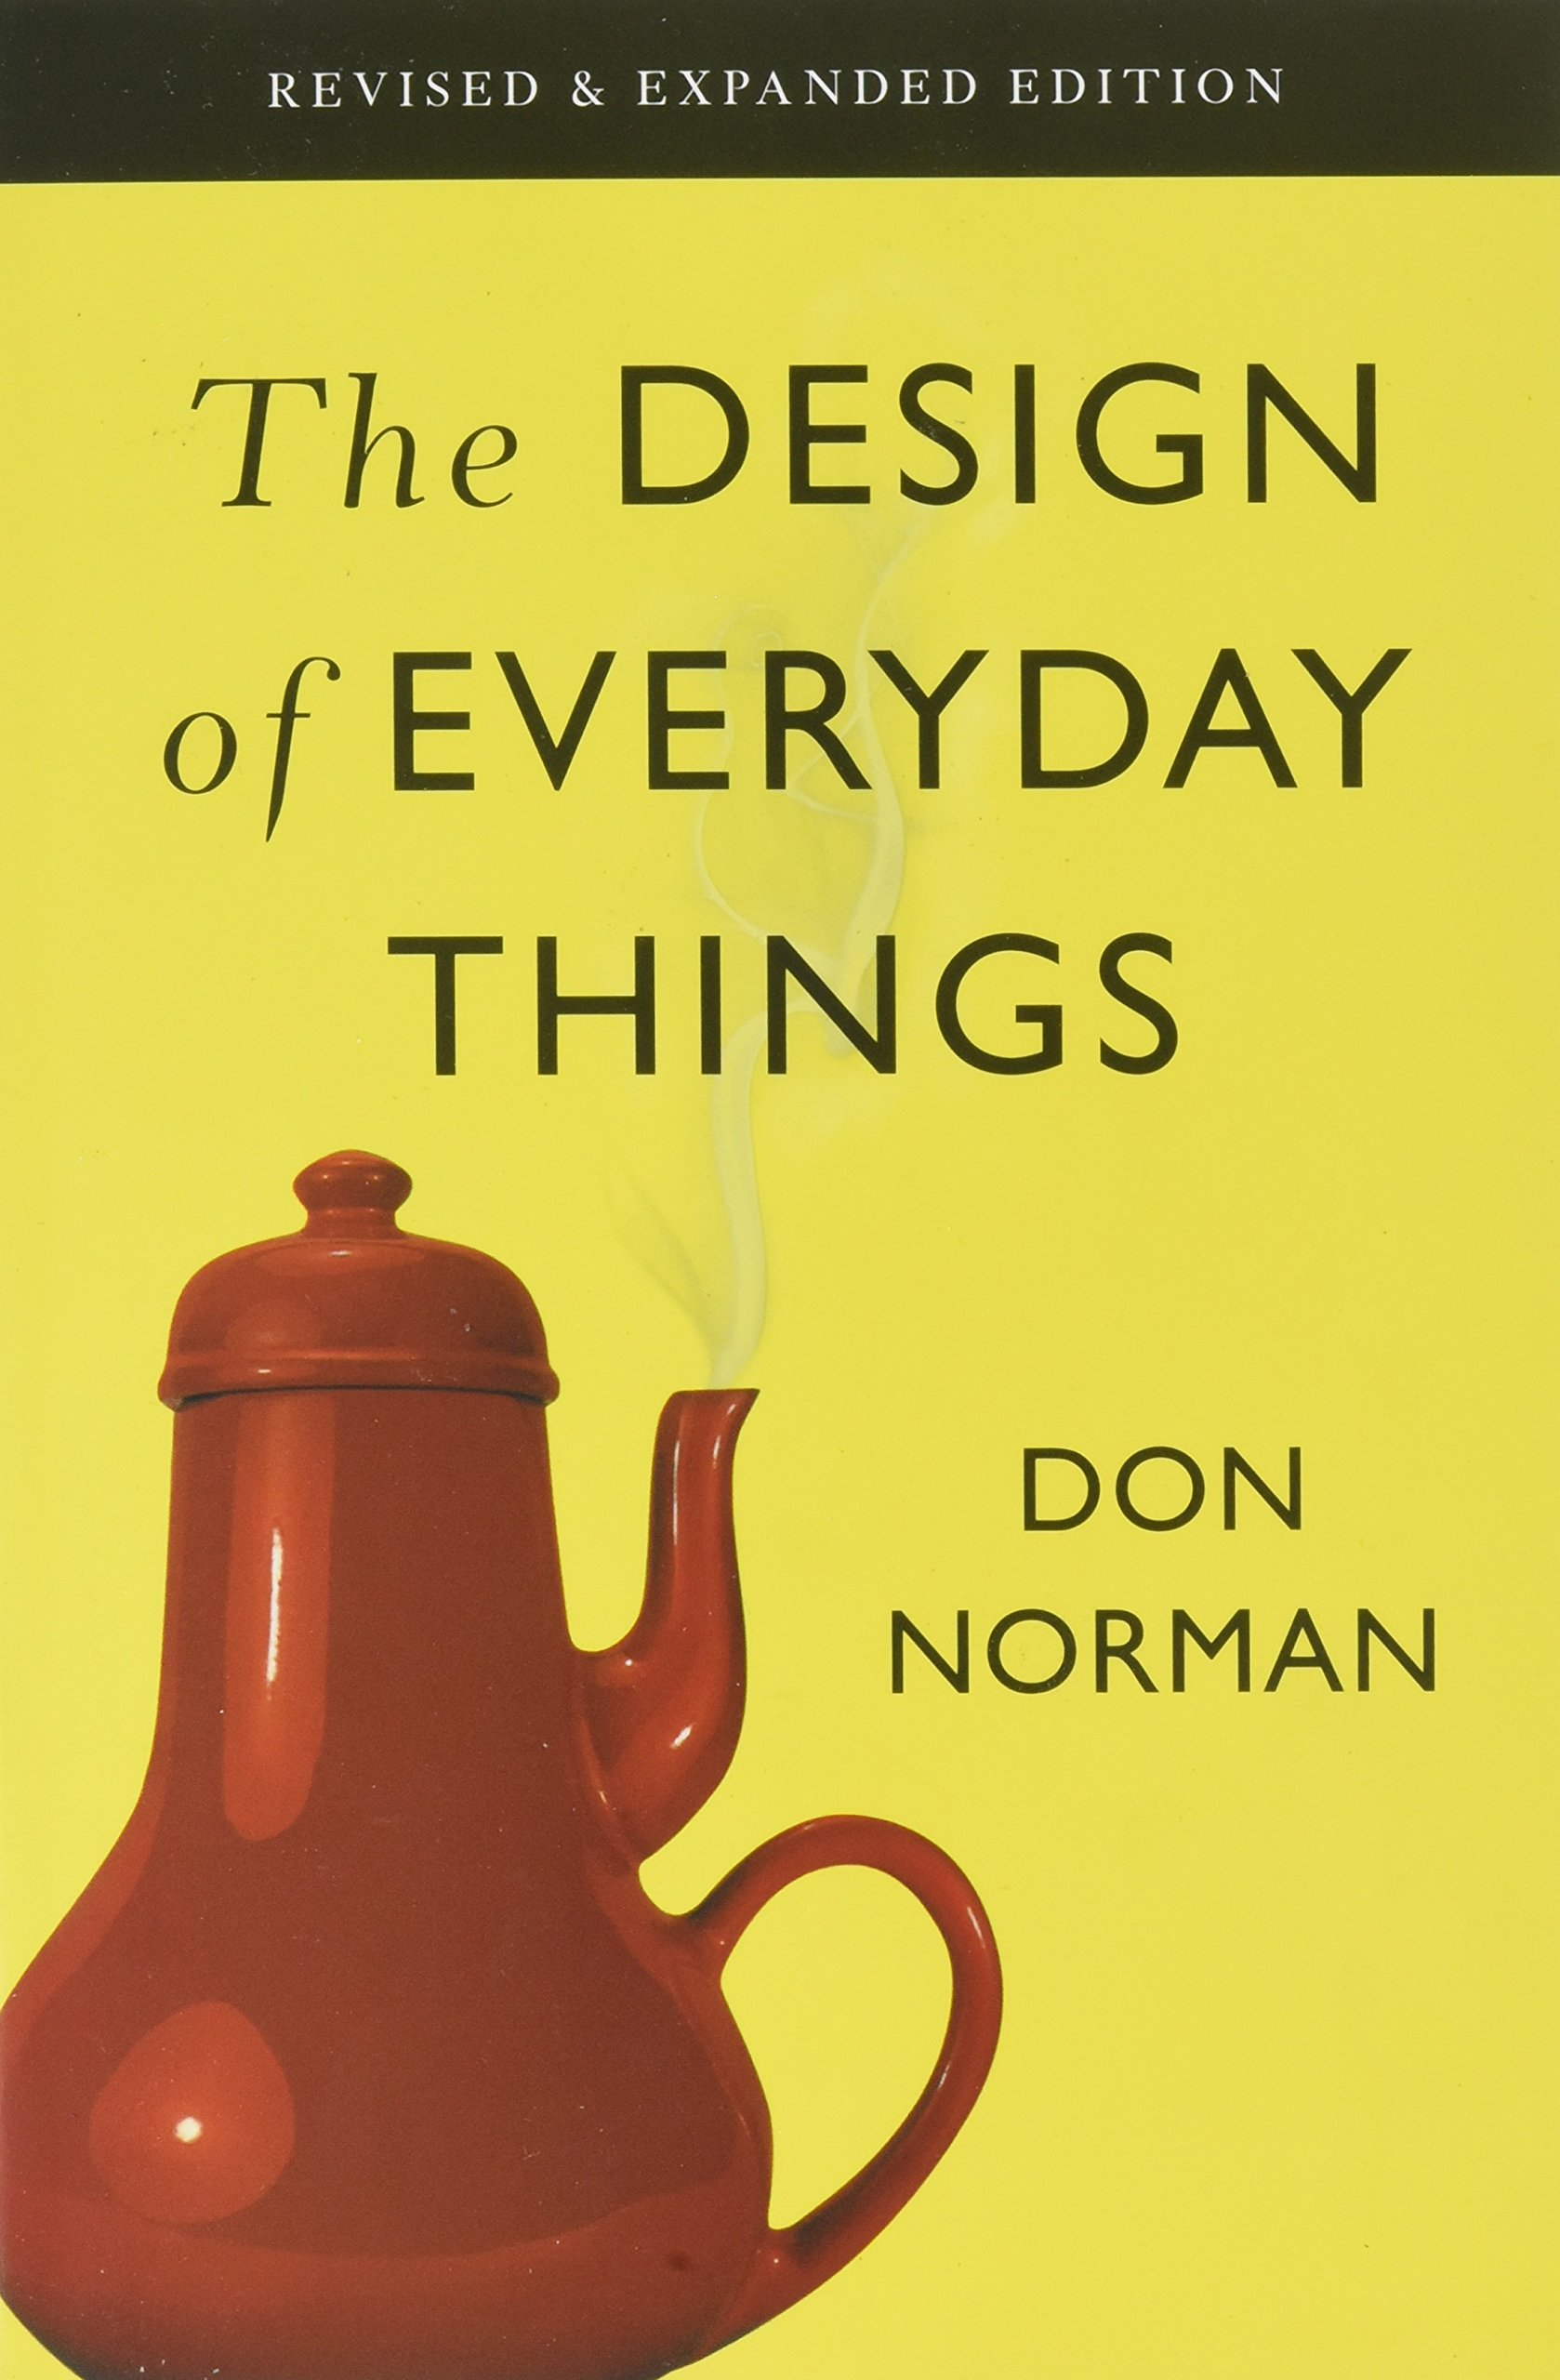
\includegraphics[width=0.8\linewidth]{norman}
			\caption{The Design of Everyday Things by Norman, Revised and Expanded ed. (2013)}
		\end{figure}
		
		\column{.32\textwidth} % Left column and width
		\begin{figure}
			
\includegraphics[width=1\linewidth]{lazar}
			\caption{Research Methods in Human-Computer Interaction by Lazar, 1st ed. (2010)}
		\end{figure}
		
		\column{.32\textwidth} % Left column and width
		\begin{figure}
			
\includegraphics[width=0.9\linewidth]{rogers}
			\caption{Interaction Design: Beyond Human Computer Interaction by Preece, Sharp and Rogers, 4th ed. (2015)}
		\end{figure}
	
	\end{columns}
	
\end{frame}

\begin{frame}
	\frametitle{Supplementary Textbooks}
	
	\begin{columns}[t] % The "c" option specifies centered vertical alignment while the "t" option is used for top vertical alignment
		
		\captionsetup{justification=centering}
		
		
		\column{.32\textwidth} % Left column and width
		\begin{figure}
			
			
\includegraphics[width=0.8\linewidth]{think}
			\caption{Don't Make Me Think by Krug, 2nd ed. (2006)}
		\end{figure}
		
		\column{.32\textwidth} % Left column and width
		\begin{figure}
			
\includegraphics[width=1\linewidth]{shneiderman}
			\caption{Designing the User Interface by Shneiderman et al., 6th ed. (2016)}
		\end{figure}
	
		
	\end{columns}
	
\end{frame}

\begin{frame}
	\frametitle{Coming Next}
	\begin{itemize}
		\item Mackenzie, Chapter 1, \textbf{History Context}, Human Computer Interaction: An Empirical Research Perspective, 1st ed. (2013) 
		\item Shneiderman, \textbf{Direct Manipulation: A Step Beyond Programming Languages} (1983)
		\item Macintosh 128K, \url{https://en.wikipedia.org/wiki/Macintosh_128K}
	\end{itemize}
\end{frame}
%------------------------------------------------

%\begin{frame}
%\frametitle{Blocks of Highlighted Text}
%\begin{block}{Block 1}
%Lorem ipsum dolor sit amet, consectetur adipiscing elit. Integer lectus nisl, ultricies in feugiat rutrum, porttitor sit amet augue. Aliquam ut tortor mauris. Sed volutpat ante purus, quis accumsan dolor.
%\end{block}
%
%\begin{block}{Block 2}
%Pellentesque sed tellus purus. Class aptent taciti sociosqu ad litora torquent per conubia nostra, per inceptos himenaeos. Vestibulum quis magna at risus dictum tempor eu vitae velit.
%\end{block}
%
%\begin{block}{Block 3}
%Suspendisse tincidunt sagittis gravida. Curabitur condimentum, enim sed venenatis rutrum, ipsum neque consectetur orci, sed blandit justo nisi ac lacus.
%\end{block}
%\end{frame}

%------------------------------------------------

%\begin{frame}
%\frametitle{Multiple Columns}
%\begin{columns}[c] % The "c" option specifies centered vertical alignment while the "t" option is used for top vertical alignment
%
%\column{.45\textwidth} % Left column and width
%\textbf{Heading}
%\begin{enumerate}
%\item Statement
%\item Explanation
%\item Example
%\end{enumerate}
%
%\column{.5\textwidth} % Right column and width
%Lorem ipsum dolor sit amet, consectetur adipiscing elit. Integer lectus nisl, ultricies in feugiat rutrum, porttitor sit amet augue. Aliquam ut tortor mauris. Sed volutpat ante purus, quis accumsan dolor.
%
%\end{columns}
%\end{frame}

%------------------------------------------------
%\section{Second Section}
%%------------------------------------------------
%
%\begin{frame}
%\frametitle{Table}
%\begin{table}
%\begin{tabular}{l l l}
%\toprule
%\textbf{Treatments} & \textbf{Response 1} & \textbf{Response 2}\\
%\midrule
%Treatment 1 & 0.0003262 & 0.562 \\
%Treatment 2 & 0.0015681 & 0.910 \\
%Treatment 3 & 0.0009271 & 0.296 \\
%\bottomrule
%\end{tabular}
%\caption{Table caption}
%\end{table}
%\end{frame}

%------------------------------------------------

%\begin{frame}
%\frametitle{Theorem}
%\begin{theorem}[Mass--energy equivalence]
%$E = mc^2$
%\end{theorem}
%\end{frame}

%------------------------------------------------

%\begin{frame}[fragile] % Need to use the fragile option when verbatim is used in the slide
%\frametitle{Verbatim}
%\begin{example}[Theorem Slide Code]
%\begin{verbatim}
%\begin{frame}
%\frametitle{Theorem}
%\begin{theorem}[Mass--energy equivalence]
%$E = mc^2$
%\end{theorem}
%\end{frame}\end{verbatim}
%\end{example}
%\end{frame}

%------------------------------------------------

%\begin{frame}
%\frametitle{Figure}
%Uncomment the code on this slide to include your own image from the same directory as the template .TeX file.
%%\begin{figure}
%%\includegraphics[width=0.8\linewidth]{test}
%%\end{figure}
%\end{frame}

%------------------------------------------------

%\begin{frame}[fragile] % Need to use the fragile option when verbatim is used in the slide
%\frametitle{Citation}
%An example of the \verb|\cite| command to cite within the presentation:\\~
%
%This statement requires citation \cite{p1}.
%\end{frame}

%------------------------------------------------

%\begin{frame}
%\frametitle{References}
%\footnotesize{
%\begin{thebibliography}{99} % Beamer does not support BibTeX so references must be inserted manually as below
%\bibitem[Smith, 2012]{p1} John Smith (2012)
%\newblock Title of the publication
%\newblock \emph{Journal Name} 12(3), 45 -- 678.
%\end{thebibliography}
%}
%\end{frame}

%------------------------------------------------

\begin{frame}
\Huge{\centerline{Questions}}
\end{frame}

%----------------------------------------------------------------------------------------

\end{document} 
